\documentclass[a4paper,10pt]{scrartcl}[2003/01/01]
\usepackage[ngerman]{babel}
\usepackage[T1]{fontenc}

\usepackage{inputenc}
\usepackage{graphicx}
\usepackage{listings}
\usepackage{enumerate}
\usepackage{pstricks}
\title{Software Architectures}
\subtitle{Exercise 6}
\author{ Felix Baumann \\ Manuel Gottschlich \\  Alexey Gy\"ori 352678 \\ Vincent Wehrwein \\ Markus Weller 352466}
\begin{document}
    \maketitle
    
    \section*{Aufgabe 6.1}
        \subsection*{a)}
        Datatypes:\\
        Node and Edge
        \subsection*{b)}
    \section*{Aufgabe 6.2 - code generation in Software engineering}
        \subsection*{a)}
        	\begin{itemize}
        		\item speed up development and reduce development costs
        		\item allow to easily reuse software design models for standard tasks and on different architectures
        		\item source code is easier to understand as it can be written in a "metalanguage"
        		\item No rewriting of the program necessary, only change the input
                \item Reuse of generator program
                \item Every output programm is correct, if the generator is.
        \end{itemize}
        \subsection*{b)}
        	Your goal is to design an ATM software. You want to have some common functions for different versions of ATMs. Since you have security requirements, you have to write in C, but you also want a mobile application in java. You Program a translator for your platform independent model to C source code that automatically replaces descriptions of functionality into source code blocks. You program another translator for Java, but can reuse the model.
        
        \newpage
    \section*{Aufgabe 6.3}
        \subsection*{a)}
        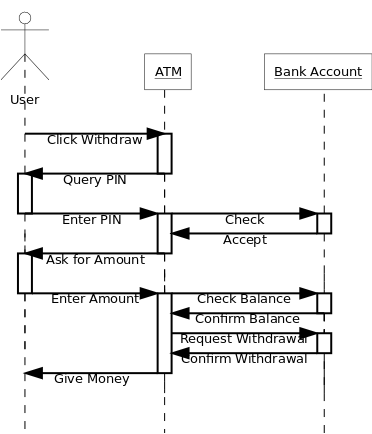
\includegraphics[scale=0.5]{Diagram1}
        \subsection*{b)}
        Sequence Diagrams are for showing complex interactions between entities.\\
        State Diagrams are for showing complex choices with the respective outcomes.\\
        
        It is hard to show different scenarios within one sequence diagram.
        \subsection*{c)}
        Class Diagrams usually only show the interfaces and variables of a class and have no information about the implementation of the functions.\\
        State and sequence are for explaining the implementation of the functions to the interfaces.
\end{document}